\RequirePackage{ifpdf}
\documentclass[a4paper,11pt]{kth-bcs}
\usepackage[T1]{fontenc}
\usepackage{textcomp}
\usepackage{lmodern}
\usepackage[utf8]{inputenc}
\usepackage[swedish,english]{babel}
\usepackage{modifications}
\usepackage{url}
\usepackage{graphicx}

\usepackage[dvipdfm,bookmarks]{hyperref}

% use sane colors for hyperlinks
\usepackage{xcolor}
\definecolor{dark-red}{rgb}{0.4,0.15,0.15}
\definecolor{dark-blue}{rgb}{0.15,0.15,0.4}
\definecolor{medium-blue}{rgb}{0,0,0.5}
\hypersetup{
    colorlinks, linkcolor={dark-red},
    citecolor={dark-blue}, urlcolor={medium-blue}
}

% enable blank pages by:
% \afterpage{\blankpage}
\usepackage{afterpage}

\newcommand\blankpage{%
    \null
    \thispagestyle{empty}%
    \addtocounter{page}{-1}%
    \newpage}

% Define a new pagestyle called 'center'
\makepagestyle{center}
\makeevenfoot{center}{}{\thepage}{}
\makeoddfoot{center}{}{\thepage}{}

\DeclareGraphicsExtensions{.eps}
%\DeclareGraphicsExtensions{.png}

\title{Configuration and device identification on network gateways}

\subtitle{Konfiguration och enhetsidentifiering på nätverksgateways}
\foreigntitle{Konfiguration och enhetsidentifiering på nätverksgateways}
\author{Simon Kers}
\date{May 2013}
\blurb{Bachelor's Thesis at KTH\\
       School of Technology and Health\\
       Supervisor: Micael Lundvall\\
       Examiner: Ibrahim Orhan
%       Kungliga Tekniska Högskolan\\
%       Skolan för teknik och hälsa\\
%       136 40 Handen, Sweden\\
%       http://www.kth.se/sth
}

\trita{TRITA-STH 2013:22}

\begin{document}

\frontmatter
\pagenumbering{roman}
\setcounter{page}{1}
\pagestyle{center}

\maketitle
\thispagestyle{center}
\selectlanguage{english}
% $#@! sammanfattningen är lite kortfattad
\begin{abstract}
   %why do we care about the problem?
To set up port forwarding rules on network gateways, certain technical skills are required from end-users.
These assumptions in the gateway software stack, can lead to an increase in support calls to the network operators and resellers of equipment.
The user interface itself is also an important part of the product and a complicated interface will contribute to a lessened user experience.
Other risks with an overwhelming user interface include faulty configuration by the user, leaving the network vulnerable to attacks.

   %what did you actually do to get your results?

   %what did you learn/invent/create?
We present an enhancement of the current port forwarding settings, with an extensible library of presets.
To help users with detecting available services, a wrapper for a network scanner was implemented, to detect devices and services on the local network.
These parts combined relieves end-users of looking up forwarding rules for ports and protocols to configure their gateway, basing their decisions on data collected by the network scanner or by using an applications name instead of its ports.

   %what are the larger implications of your findings
Using the Nmap utility for identifying services on the network, could be considered harmful activity by network admins and intrusion detection systems.
The preset library is extensible and generic enough to be included in the default software suite shipping with the network equipment.
Working within the centralized configuration system within OpenWrt, the preset design will add value and allow resellers to customize their services.
This proposal could reduce support costs for the service operators and improve user experience and configuration of network gateways.

\end{abstract}
\newpage
\blankpage

\begin{foreignabstract}{swedish}
Vid vidarebefodring av portar i nätverksgateways, krävs ibland vissa tekniska förkunskaper av användaren.
De höga kraven på kunskapsnivå kan bidra till ett ökat antal supportsamtal för återförsäljare och nätverksoperatörer.
Användargränssnittet i sig är också en viktig del i produkten och ett komplicerat gränssnitt bidrar till försämrad användarupplevelse.
%Other risks with an overwhelming user interface include faulty configuration, leaving the network vulnerable to attacks.
Övriga problem med komplicerade användargränssnitt är risken för felaktig konfiguration, vilket kan utsätta nätverket för attacker.

%We present an enhancement of the current port forwarding settings, with an extensible library of presets.
En förbättring av nuvarande \emph{port forwarding}-inställningar presenteras, tillsammans med ett utbyggbart bibliotek med förinställda regler.
%To help users with detecting available services, a wrapper for a network scanner was implemented, to detect devices and services on the local network.
För att hjälpa användare att identifiera enheter och sätta rätt inställningar, utvecklades en wrapper för en portskanner, vilken kan identifiera enheter och nättjänster i den lokala nätverket.
%These parts combined relieves end-users of looking up forwarding rules for ports and protocols to configure their gateway, basing their decisions on data collected by the network scanner or by using an applications name instead of its ports.
Tillsammans underlättar dessa delar för slutanvändare, befriar dem från att referera till regler för portar och protokoll och möjliggör inställning enbart genom att använda portskanning eller välja namnet på tjänsten från en lista.

%Using the Nmap utility for identifying services on the network, could be considered harmful activity by network admins and intrusion detection systems.
Användandet av verktyget Nmap för att identifiera nättjänster på nätverket kan möjligtvis betraktas som dataintrång av nätverksadministratörer och intrångdetekteringssystem.
%The preset library is extensible and generic enough to be included in the default software suite shipping with the network equipment.
Databasen med förinställningar är utbyggbar, fungerar och passar in tillräckligt bra för att innefattas i standardmjukvaran.
%Working within the centralized configuration system within OpenWrt, the preset
%design will add value and allow resellers to customize its services.
Via det centraliserade konfigurationssystemet i OpenWrt, kommer utformningen av systemet med förinställningar för port forwarding möjliggöra för komplementering av nättjänster och enheter från återförsäljare. 
%This proposal could reduce support costs for the service operators and improve user experience and configuration of network gateways.
Systemet kan minska supportkostnader för bredbandsleverantörer och bidra till en förbättrad användarupplevelse vid konfiguration av nätverksgateways.

\newpage
\blankpage

\end{foreignabstract}
\clearpage
\tableofcontents*
\mainmatter
\pagestyle{newchap}
\chapter{Introduction}
%brief introduction to inteno and the product
%\section{Background}
Inteno Broadband Technology is a company that supplies \emph{customer premises equipment} (CPE) for internet service providers.  
Their headquarters and \emph{research and development center} is located in Stockholm, Sweden.
Inteno Open Systems Platform, or \emph{iopsys}, is a Linux-based open source platform running on their CPE.
It is based on the OpenWrt distribution which targets embedded devices, specifically network gateways.\cite{Inteno}

%identified a real problem (motivate that it is real and interesting)
The technical support departments of partners and resellers of Inteno CPE, are looking to reduce support costs and improve customer experience. 
Support issues creates costs for the business and by reducing the number of support tickets and their processing time, these costs can be reduced.

\section{Goals}
%come up with a solution (give a rough idea what the solution looks like)
By simplifying configuration through abstracting common tasks for the end-user, the number of support calls can be reduced.
Using automatic device identification and automating common tasks such as port forwarding, will also lead to savings in support along with a better user experience.
Many common support issues could be automated by the software running on the CPE and by effective communication with the end-user through the user interface, these improvements would also aid first-line support when guiding the customer over phone.

\begin{itemize}
   \item Preset library of port forwarding rules
   \item Automatic detection of services on the local network devices
   \item Internal DNS translation of the gateway IP address
\end{itemize}

\section{Definition}
To reduce the amount of support calls, a feature of automatic service discovery on the local network would be developed, achieving a more user friendly operation.
A system that identifies the ports and services running on the network devices, that the end-user might want to set up forwarding rules for.

\section{Solutions}
%how I actually solved the problem (high-level summary of results).
By building a library of presets for common port forwarding rules and developing a simple selection dialog, the end user can more efficiently set up port their firewall redirection rules and general configuration of their gateway.
A limited range of settings and helpful hints are presented in the forwarding dialog.

The system for service identification is a wrapper around \emph{Nmap}, that performs a scan of the network nodes and returns a list of available services.
This information is in turn used to match against the known presets and protocols, and offer the user a choice of applying the preset rules for the newly detected network device.
%skriv klart angående att tack vare ramverket så kan åf lägga till egna regler.
The preset system is extensible, allowing retailers to add their own devices and services as preset definitions, each with their specific forwarding rules.

DNS translation of the gateway IP address, allows easy access through the web browser by simply entering a word in the address bar, which should be easier for users than remembering or figuring out its IP.

%\part{Important Results}

\chapter{Background}

The research and development department at Inteno works on improving the platform, adding value to the end users, the operators and the larger OpenWrt software ecosystem.
Because of the nature of OpenWrt's free software licence\footnote{GNU General Public License is a ``free as in freedom'' software licence}, the code is publicly released and available for download from Intenos webpage\cite{inteno_gpl}.

There are simple ways in which to improve the user experience, developers of network gateway software often implement a set of presets of port forwarding rules for common applications.
The interface presents the user with a list of applications in plain text and lets the user select an IP address, for which the forwarding rules should apply.

Alternative solutions to simplifying port forwarding include using standalone applications which run on a PC, connected to the local network.
These applications has internal lists of port forwarding rules for common applications and devices, which is then applied for a specific IP address on the local network.
\cite{portforward.com}


\chapter{Theory}
%skriv något om alternativa program typ port forwarding
%skriv möjligtvis något om alt. till Nmap, kanske p0f bör nämnas?

%skriv något om alternativa program typ port scanner och guider på nätet
To test the newly applied configurations, web-based or locally run port scanners can be used.
They will scan the users external IP address for open ports and present which are open, this does not guarantee that the packets are routed to the correct internal address.

\section{Programming languages}
\subsection{Lua}
Lua is a programming language that is intended to be embeddable and extensible, it is implemented in C and enables the developer to employ different programming techniques with its multi-paradigm approach.
The programming languages it is distributed with a permissive free software licence\cite{mit-license}, while being open source allowing use within proprietary software.
The language is dynamically typed, which means that the underlying variable type is determined at runtime and supports features such as memory management, closures and first-class functions.\nocite{ierusalimschy2006programming}
%motivera valet av Lua, Model-View Controller framework LuCI använder Lua?

Since the web user interface of OpenWrt uses Lua, it was beneficial to implement as much of the application in the programming language, as a Lua Configuration Interface module.
See section \ref{sec:LuCI} for details on \emph{Lua Configuration Interface}, or LuCI.

\subsection{Almquist shell}
Adhering to the POSIX standards, Almquist shell\footnote{Also called \emph{sh}, \emph{A shell} or \emph{ash}} on OpenWrt it is the default operating system command-line interface, scripting language and command processor.
It has less features than \emph{bash} and sometimes requires a strict and sometimes more verbose scripting style, without the permissiveness of bash idioms, such practices are referred to as \emph{bashism} and are often incompatible with ash.

Shell scripting allows the developer to aggregate the power of a range of UNIX programs, using redirection to route the output of one program to the input of another, and with the shell prompt as an interactive development environment it allows for rapid prototyping.
The permissiveness and features of bash, has brought along handy constructs such as \emph{process substitution}, which is unavailable in ash.
Instead the developer has to resort to manually handling named pipes, which creates a temporary buffer in which the processes can exchange data.
An example redirecting the output from a command a named pipe, and processing the output of that command is available in appendix \ref{fig:fifo}.

\section{Software suite}

The newer Inteno devices ship with the OpenWrt distribution, which is a small GNU/Linux operating system.
It provides the developer with the basic UNIX debugging tools and a POSIX compatible command-line interface shell.
As common with free software, the OpenWrt exists in an ecosystem of applications and tools, in this chapter a few of these parts are discussed.

\subsection{OpenWrt}
OpenWrt is a free and open-source GNU/Linux distribution, targeting embedded devices, specifically wireless routers, but can run on almost any set of hardware.
Cross-compilation is enabled by OpenWrt Buildroot, which compiles the C code using uClibc, a lightweight C library focusing on embedded Linux systems. 
It intends to be a meta distribution and offers developers a framework on which to base their firmware on.

OpenWrt is generally compiled and linked using gcc and binutils, with the help of Makefiles and patches for the various gcc versions and target platforms.
Allowing end users as well as service operators and hardware manufacturers to compile the firmware.
It offers the BusyBox set of barebones UNIX tools, enabling advanced users to fully interact with their Linux system and providing developers with a familiar platform for debugging and testing their product.
\cite{OpenWrt:structure_design}

\emph{Unified Configuration Interface}, or UCI, is used in OpenWrt as a uniform format for commonly used configuration files.
UCI has a Lua bindings as well as a command line interface, to read and modify the configuration files.
Rules for port forwarding are defined in the UCI compatible configuration file in:
\begin{verbatim}
    /etc/config/firewall
\end{verbatim}

A port forwarding rule which forwards external HTTP traffic over port 80 to the internal IP 192.168.1.214, is shown in figure \ref{fig:redirect_conf} in appendix \ref{appA}.
The line \emph{config redirect} defines the start of a section, a section contains several values and a UCI configuration file can have several such sections.

\subsection{OPKG}
The package management system used in OpenWrt is Open PacKaGe Management, or \emph{OPKG}. It is based off the discontinued \emph{ipkg} and operates similar to \emph{APT} and \emph{dpkg} of Debian-based distributions.
It targets GNU/Linux based operating systems for embedded devices and there are currently over 2000 OPKG packages available for OpenWrt.

The OpenWrt system and its packages are built using \emph{GNU Autoconf}, which automates tasks associated with compiling larger software suites.
This includes pulling in parts of the system from remote software repositories and automatically resolving dependencies on programs and libraries.

\subsection{Inteno Open Platform System}
For Customer Premises Equipment like wireless gateways, Inteno Open Platform System offers an open-source Linux distribution based on OpenWrt.
It uses the OpenWrt build system including cross-compilation toolchain to ensure compatibility with the ecosystem and upstream.

Inteno maintains and hosts a remote repository, which contains a frozen release of OpenWrt and compatible packages and patches.
Freezing an ever changing open source codebase means forking an existing version, submitting more conservative patches to the system and focusing on smaller changes.
This leads to good compatibility with Inteno hardware and protection from breakage because of upstream\footnote{Code released and maintained by the official project} code changes.

\subsection{Lua Configuration Interface}\label{sec:LuCI}
Lua Configuration Interface, or \emph{LuCI}, is a suite of programs and libraries for extending OpenWrt using the Lua programming language and providing a web interface built with the Model-View Controller architecture.
It originated in the OpenWrt project, but is now an independent project on its own.


\subsection{Model-View Controller}
LuCI relies on the \emph{Model-View Controller} software architecture pattern and separates data and its visual representation.
It is divides in three parts with the model representing the data and storing in in UCI configuration files.

\chapter{Problem}
   \section{User experience}
End users of Inteno CPE have expressed concern about the relative difficulty of port forwarding and configuration of their network gateway.
The default settings page for port forwarding is currently located under the \emph{Firewall} tab in the OpenWrt front end, the forwarding procedure involves looking up ports for the specific device or unit, and entering these on the web page forms.

These set of rules sometimes involve several ports and protocols, increasing the possibility for misstep and faulty configuration by the end user.
If we could reduce the complexities of this common task of address translation and present it in an way that are easily understandable, then customer satisfaction would increase.
Such tasks could be well suited for automation by software, especially for applications and devices which require several port forwarding rules, automating some of these steps will save time and bring overall value to the user experience.


   \section{Customer support}
Connectivity of the XBox 360 gaming console has been a common issue and the device is common among end users, this was also chosen as reference device to do tests and verifications against.
One of the most commonly reported issues of end users, is setting up port forwarding for connecting their XBox 360 to the XBox Live network.

\chapter{Design}

The overall design of the system consists of two parts, the service identification and port forwarding presets.
These parts are connected through the underlying software and presented on the user interface.

As shown in figure~\ref{fig:wizard-seq_dia}, the communication between the parts of the port forwarding process is outlined.
The user initiates the identification procedure and the identification process starts.
When the results from the identification are returned the list of presets is sorted, based on identification and the user can review their options.
By selecting the name of the service, the correct forwarding rules are loaded and presented to the user, who can then chose to apply them, after which they are written to the configuration files.
\begin{figure}[h!]
   \centering
   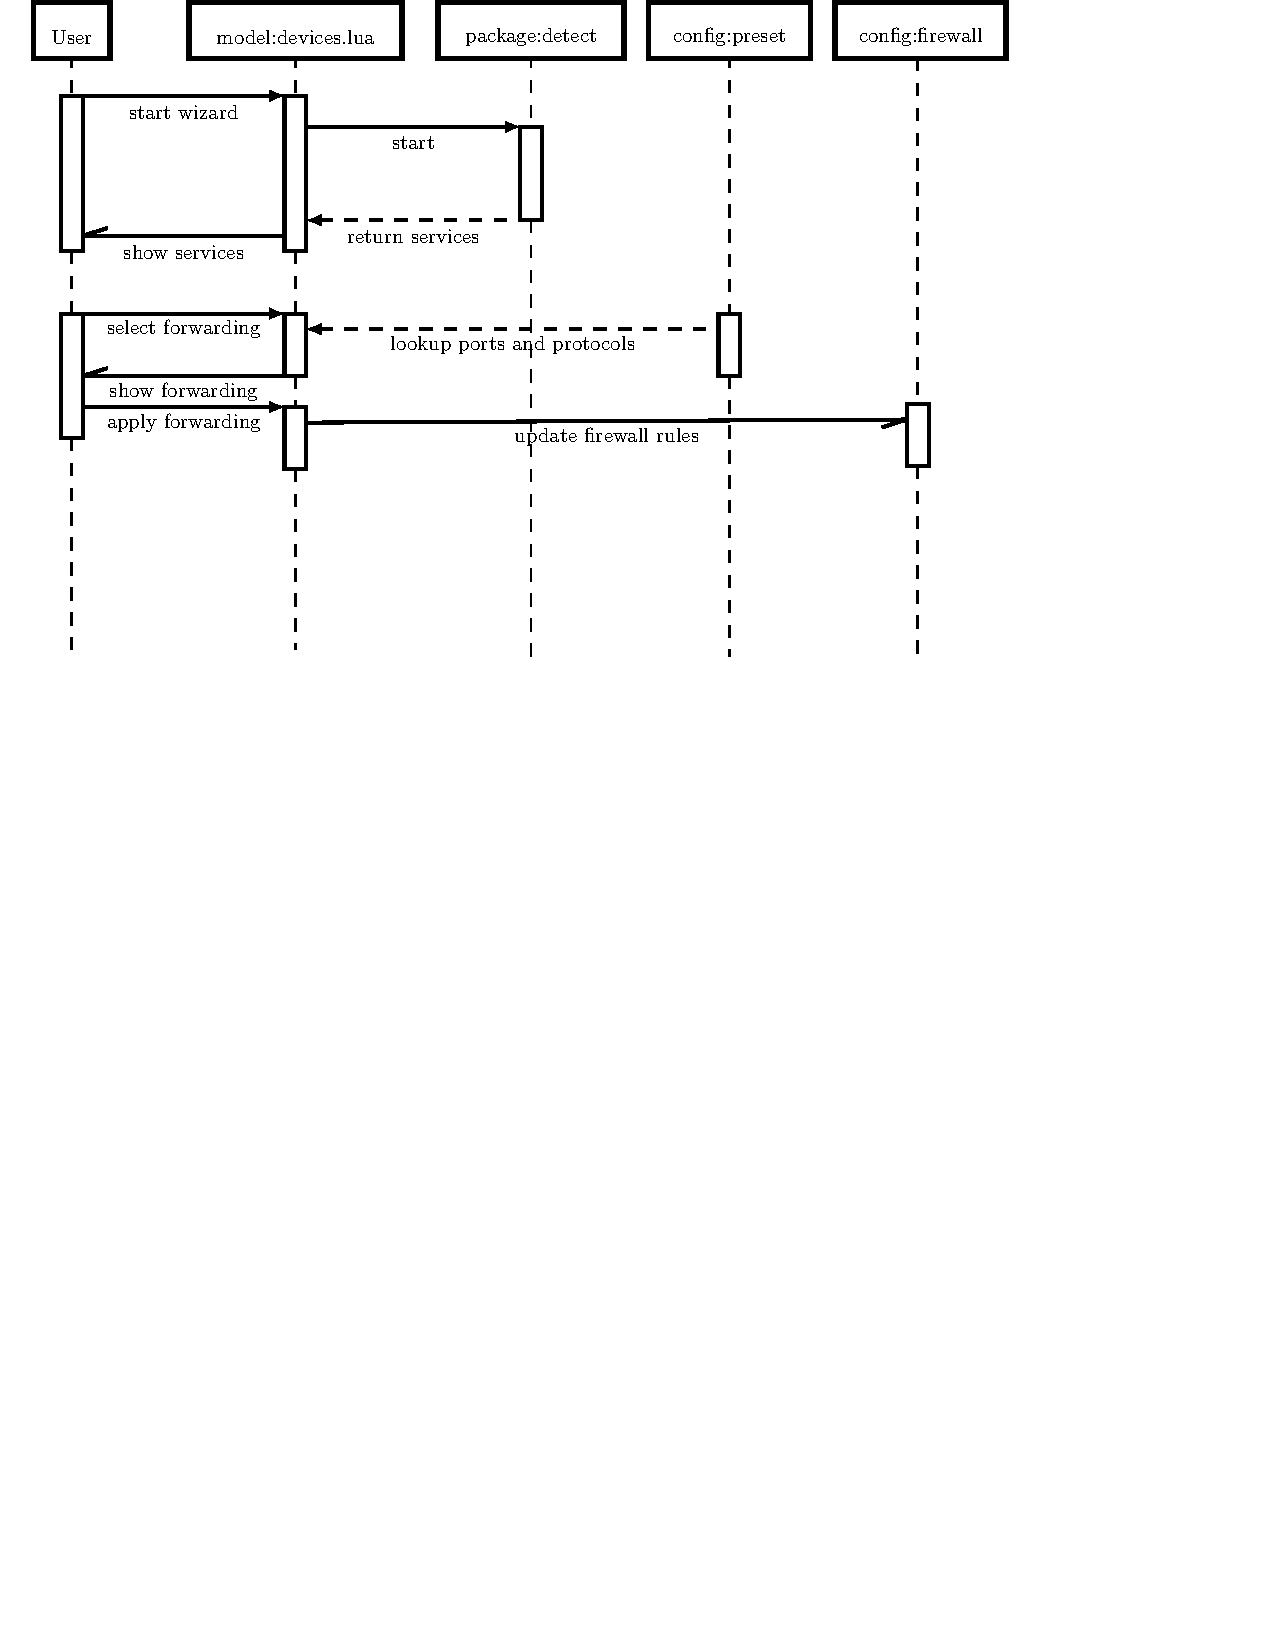
\includegraphics[width=15cm]{wizard-seq_dia}
   \caption{Sequential diagram of applying port forwarding rules}
   \label{fig:wizard-seq_dia}
\end{figure}
%   \section{Human-computer interaction}
%This is a cite\cite{garrett2003elements}

   \section{User interface}
For a port forwarding interface page, the user is presented with detected nodes and their respective network services.
Listed presets are sorted by the output from the service identification process, presenting the user with the most likely services at the top of the list.

To apply the port forwarding rule set, the user selects a node in the network and the service from the sorted list, then applies it.
Instead of performing all the steps automatically, the user is required to interact and approve of the suggested changes.
The service identification is there to help the users make choices, not deciding for them.

\chapter{Implementation}
%explain your approach in a general overview
The implementation consists of three general parts that work together in delivering easier forwarding rules configuration.
As shown in figure~\ref{fig:wizard-seq_dia}, the three configuration files that together with user input, are used as sources for the final redirection rule in the firewall configuration file.
The device detection updates the configuration file \emph{devices} with newly discovered devices, this does not include applications running on computers or game specific forwarding rules, running on gaming consoles, this requires user intervention.

%The OpenWrt distribution provides a complete platform for compiling and deploying a gateway firmware image.

% $#@! Jag kan inte hitta hur metodval för att lösa uppgiften har gjorts. Du använder dig av Nmap och en Wrapper, men undersökte du andra möjligheter och varför fasnade du i sådana fall för just den här lösningen? 
\section{Nmap}
The program \emph{Nmap} is a popular network discovery program, and was chosen as the engine for the service scanner implementation.
The XBox 360 gaming console was chosen at Inteno's suggestion, with the motivation that it is one of the devices that end users have had the most issues with, in regards to port forwarding.
Nmap is capable of detecting several operating systems, embedded devices and network services.
%skriv något om probes, fingerprinting och teknikerna som används för id

Using Nmap is quite intrusive and could be detected as an attack by intrusion detection software, used to monitor the network for illicit behavior.
An alternative approach is using passive fingerprinting of network traffic, one such utility if P0f which uses passive scanning of traffic.\cite{p0f}
Inteno routers are configured with cut-through switching, which effectively hides the packet information from software processing and analyzing techniques.

\subsection{Wrapper}
Executing the Nmap scanning utility and returning results, is implemented as a shell script.
%skriv att du valde att göra shellhax istället för Lua
In the development process of the wrapper, a shell script was written to test the functionality and extract data about the detected services.
The original thought was to replace this with a Lua script, to make it more cohesive with the rest of the system.
Due to lack of time, the rewrite was cancelled and a quick adaptation was made to to the script to return valid JSON for the JavaScript frontend.

% $#@! Det vore även upplysande att se ett exempel på resultatet av en sådan extrascanning som beskrivs längst ned på sidan 11 alternativt hänvisa till information som du presenterar i Appendix.
%discuss tradeoffs, discuss traps you've fallen into
%skriv att xbox inte hittas och att du var tvungen att haxa
While testing the service identification features of Nmap, there is no way for Nmap to positively identify an XBox 360.
This failure was due to an inconclusive fingerprint, but using the flag called version scan -- run with arguments \emph{-sV} -- Nmap interrogates ports and returns more information than a regular operating system scan.
The extra scan using the Nmap \emph{version scan}, was successfully used to identify the XBox 360.
Whenever the service is identified as \emph{LSA-or-nterm}, the TCP ports 1026 and 1027, were scanned, either of these are in use by the XBox 360.\cite{aretheysecure}
The more thorough version scan is then matched for \emph{XBox 360 UPnP}, which the wrapper is set to interpret as a positive match.
%se till att raden XBox 360 UPnP stämmer väl överens med verkligheten

\section{Preset library}
The preset library consists of common services and port data, that the user would want to set up forwarding rules for.
Details of these ports and protocols are provided by the application developers, specifically for address translation reasons.

%explain your design and limitations in greater detail
Using the \emph{Unified Configuration System}, that is included in the OpenWrt distribution, all the basic commands for configuring the firewall rules were prototyped and explored.
A set of \emph{XBox 360} port forwarding rules from the preset configuration file is shown in figure \ref{fig:redirect_conf} in appendix \ref{appA}.

The rules were formatted to fit the UCI configuration file format and returned as JSON to the JavaScript frontend in an AJAX call through the Lua dispatcher.\footnote{The dispatcher is the \emph{Controller} in the MVC framework}

Applying the rules requires the user to select the desired service from a list, and pressing a button which runs a JavaScript function, performing an AJAX call to the Lua backend, issuing the UCI calls.

%\section{Dispatching commands}

\chapter{Results}
% $#@! Jämför även gärna med resultatet av en normal scanning.

%lägg till resultat från scanningen med tid och exempel
Scanning a Raspberry Pi installed with the options \emph{web server}, \emph{mail server} and \emph{ssh server}, detect these services and ports as shown in figure \ref{fig:rasp_scan}.
The mail server option in the installer, enables identification on ports 110, 143, 993 and 995 because of the various email delivery protocols.

   \begin{figure}[ht]
      \centering
      \label{fig:rasp_scan}
\begin{verbatim}
   PORT    STATE SERVICE  REASON  VERSION
   22/tcp  open  ssh      syn-ack OpenSSH 6.0p1 Debian 4 (protocol 2.0)
   80/tcp  open  http     syn-ack Apache httpd 2.2.22 ((Debian))
   110/tcp open  pop3     syn-ack Dovecot pop3d
   111/tcp open  rpcbind  syn-ack 2-4 (RPC #100000)
   143/tcp open  imap     syn-ack Dovecot imapd
   993/tcp open  ssl/imap syn-ack Dovecot imapd
   995/tcp open  ssl/pop3 syn-ack Dovecot pop3d
   MAC Address: B8:27:EB:0C:A5:70 (Raspberry Pi Foundation)
\end{verbatim}
      \caption{
         \small{
Nmap version scan of the Raspberry Pi, identifying available services on the open ports.
         }
      }
   \end{figure}
The front-end with select the first service from the dropdown list of presets and present the user with the choice to apply its forwarding rules.

\newpage
\section{Operating system scan}
As shown in figure \ref{fig:nmapos}, the scan is unable to identify the correct operating system. The scan had a duration of 43.74 seconds.

   \begin{figure}[ht]
      \centering
      \begin{verbatim}
root@Inteno:~# time nmap -O --osscan-guess --fuzzy 192.168.1.218

Starting Nmap 5.51 ( http://nmap.org ) at 2013-05-28 18:03 CEST
Nmap scan report for 192.168.1.218
Host is up (0.00061s latency).
Not shown: 999 filtered ports
PORT     STATE SERVICE
1026/tcp open  LSA-or-nterm
MAC Address: 00:22:48:40:11:FE (Microsoft)
Warning: OSScan results may be unreliable because we could not find at least 1
open and 1 closed port
Device type: general purpose|switch
Running (JUST GUESSING): IBM OS/2 4.X (92%), HP OpenVMS 7.X|8.X (88%), HP embedded
(87%), Fujitsu Siemens ReliantUNIX (86%), Compaq Tru64 UNIX 5.X (85%)
Aggressive OS guesses: IBM OS/2 Warp 2.0 (92%), HP OpenVMS 7.2 (88%), HP ProCurve
2524 switch (J4813A) (87%), HP ProCurve 4104gl or 4108gl switch (87%), Fujitsu
Siemens ReliantUNIX-N (SINIX-N) on RM400 (86%), Compaq Tru64 UNIX 5.1B or HP OpenVMS
8.2 - 8.3 (85%), HP OpenVMS 8.3 (85%), HP OpenVMS 7.3 (85%), HP OpenVMS 7.2-1 (85%)
No exact OS matches for host (test conditions non-ideal).
Network Distance: 1 hop

OS detection performed. Please report any incorrect results at
http://nmap.org/submit/ .
Nmap done: 1 IP address (1 host up) scanned in 41.67 seconds
real	0m 43.74s
user	0m 19.50s
sys	0m 5.57s
      \end{verbatim}
      \caption{
         \small{
Raw output of first Nmap scan of XBox 360, failing to guess target operating system
         }
      }
      \label{fig:nmapos}
   \end{figure}

\newpage
\section{Version scan}
By issuing a version scan, this run of Nmap is able to positively identify the service \emph{XBox 360 XML UPnP (Serial number 757502283805)} in 13 seconds, as shown in figure \ref{fig:nmapxbox}.
   \begin{figure}[ht]
      \centering
      \begin{verbatim}
root@Inteno:~# time nmap -sV -p 1026-1027 192.168.1.218

Starting Nmap 5.51 ( http://nmap.org ) at 2013-05-28 18:06 CEST
Nmap scan report for 192.168.1.218
Host is up (0.00081s latency).
PORT     STATE    SERVICE VERSION
1026/tcp open     upnp    XBox 360 XML UPnP (Serial number 757502283805)
1027/tcp filtered IIS
MAC Address: 00:22:48:40:11:FE (Microsoft)
Service Info: Device: game console

Service detection performed. Please report any incorrect results at
http://nmap.org/submit/ .
Nmap done: 1 IP address (1 host up) scanned in 12.89 seconds
real	0m 13.02s
user	0m 4.09s
sys	0m 1.44s
      \end{verbatim}
      \caption{
	 \small{
       Raw output of deeper Nmap scan of XBox 360, positively identifying it with \emph{XBox 360 UPnP}
	 }
      }
      \label{fig:nmapxbox}
   \end{figure}

%\section{Performance}
%skriv ned hur lång tid det tar att scanna

\chapter{Conclusions}
%discuss what we can learn from the results
The results shows that the system manages to identify the XBox 360 gaming console, using our extension built into the wrapper.
Its services in terms of ports are well known and defined in the preset part of the implemented system.
The Raspberry Pi running the Debian GNU/Linux distribution is successfully detected as such, all services selected during the installation are successfully detected.

%draw real conclusions
The preset system will simplify the port forwarding procedure and provide the novice user with helpful hints, in an otherwise complex graphical environment.
Device and service detection fits with the preset data and the combination of these results results in a qualified guess, which is presented in the user interface.
This part of the system could be made production ready and included by default in the iopsys platform.

The identification process of the XBox 360 is not a generic Nmap solution, it requires a workaround implemented in our shell script wrapper.
This behaviour is undesirable but perhaps acceptable, depending on the frequency of the issue.
Considering the CPE operators various needs, we are unable to draw any conclusions as to weather it should be implemented or not.

\newpage
\section{Further development}
%explain how to fix shortcommings of work and how to fix them
The solution using Nmap could be interpreted as illegal activity and attempts at exploiting the systems of a network administrator, this is a risk which could render the proposed solution undesirable.
A fix for this would be to implement a less intrusive way of identifying services, reviewing the ARP tables which contains the cache of the address resolution protocol.
One could filter possible devices by their manufacturers MAC address, with an already populated ARP table this procedure is unintrusive and fast.
A more detailed Nmap \emph{version scan} could then be performed according to a configuration file, mapping MAC addresses to minimal Nmap commands.

The execution time of Nmap is an issue, on local networks with several devices the latency would be deemed too high.
To address this issue one could adjust the service to preload the automatic identification results and have it run in the background, to provide a more responsive user experience with cached results.

\newpage
\newpage
\appendix
\addappheadtotoc
\chapter{Configuration files}\label{appA}
   %\addcontentsline{toc}{section}{Configuration files}

   \begin{figure}[ht]
      \centering
      \begin{verbatim}
   config redirect               
           option target 'DNAT' 
           option src 'wan'
           option dest 'lan'
           option proto 'tcp'
           option src_dport '80'
           option dest_ip '192.168.1.214'
           option dest_port '80' 
           option name 'Web server'
      \end{verbatim}
      \caption{
         \small{
Port forwarding section in the UCI \emph{firewall} configuration file
         }
      }
      \label{fig:redirect_conf}
   \end{figure}

   \begin{figure}[ht]
      \centering
      \begin{verbatim}
   config device 'xbox360'
      option name 'xbox360'
      option description 'Xbox 360 Live'

   config redirect
      option device 'xbox360'
      option proto 'udp'
      option port '88'

   config redirect
      option device 'xbox360'
      option proto 'tcp udp'
      option port '3074'

   config redirect
      option device 'xbox360'
      option proto 'tcp udp'
      option port '53'

   config redirect
      option device 'xbox360'
      option proto 'tcp'
      option port '80'
      \end{verbatim}
      \caption{
         \small{
Preset for port forwarding sections in the UCI \emph{preset} configuration file
         }
      }
      \label{fig:preset_conf}
   \end{figure}

\chapter{Shell scripting}\label{appB}
   \begin{figure}[ht]
      \centering
      \begin{verbatim}
[ ! -p /tmp/fifo ] && mkfifo /tmp/fifo
nmap -O --osscan-guess --fuzzy $1 > /tmp/fifo &
while read -r line
do
  case "$line" in
    # perform operation on line
  esac
done < /tmp/fifo
rm /tmp/fifo
      \end{verbatim}
      \caption{
         \small{
Using a named pipe to redirect the output of one program to a temporary file and reading it line by line, performing operations.
         }
      }
      \label{fig:fifo}
   \end{figure}

\bibliographystyle{plain}
\bibliography{bibliography}
\end{document}
